\chapter{Characterisation of the calorimeter resolution}

Optical modules have been characterised before installation.
Most of the \Co\ $\beta$ desintegrations are followed by the emission of two $\gamma$s in coincidence (see Fig.~\ref{fig:Co_decay_scheme}).
The idea is to use this source to calibrate in time optical modules of SuperNEMO demonstrator by placing it behind the main calorimeter walls (the demonstrator being closed since ...) and using the two coincidence $\gamma$s.
Performing simulations of \Co\ desintegrations



\section{Calibration with a Cobalt source}
\label{sec:CoSource}

\subsection{Experimental setting and goal}
\subsection{Data taking at LSM}
\subsection{Analysis}
\subsection{Results}


\section{The Light Injection System}
\label{sec:LIS}

\subsection{Principle}
\subsection{Time resulotion of optical modules}

\begin{figure}
  \centering
  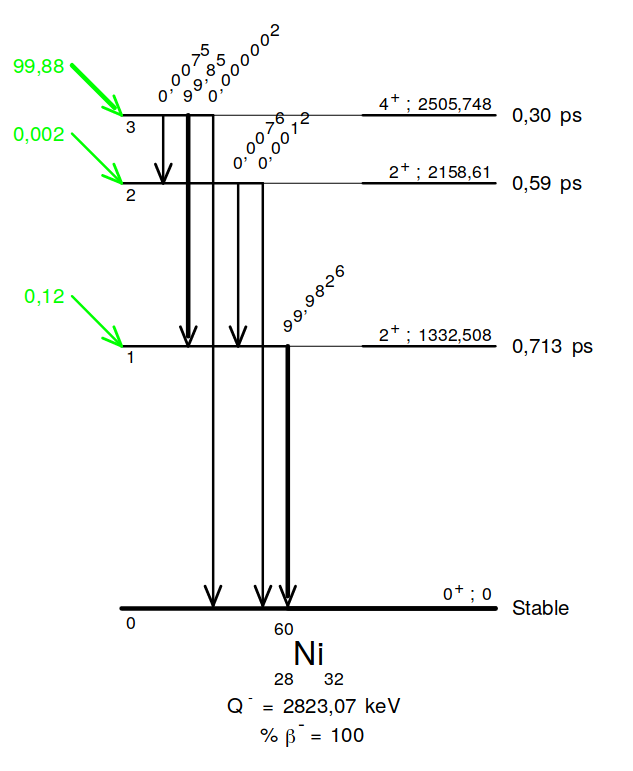
\includegraphics[width=10cm]{CoSource/fig_CoSource/Co_decay_scheme.png}
  \label{fig:Co_decay_scheme}
  \caption{Decay scheme of Cobalt $60$.
  After the $\beta$ desintegration $99.88$\%, }
\end{figure}
